\documentclass[
 aps,
 jmp,
 amsmath,amssymb,
 reprint,
]{revtex4-2}

\usepackage{graphicx}% Include figure files
\usepackage{dcolumn}% Align table columns on decimal point
\usepackage{bm}% bold math
\usepackage{mathtools}
\usepackage{amsthm,amssymb, hyperref}
\usepackage{xcolor}
\DeclarePairedDelimiter{\ceil}{\lceil}{\rceil}

\begin{document}

\preprint{AIP/123-QED}

\title[Quantum Accelerated Causal Tomography...]{Quantum Accelerated Causal Tomography: \\Circuit Considerations Towards Applications}%
\thanks{All authors contributed equally to this work.}

\author{Tamal Acharya}
\email{tamal\_974@yahoo.com}
\affiliation{QWorld Association.}
\affiliation{Purdue University, West Lafayette, USA.} 
%
\author{Akash Kundu}
\email{akundu@iitis.pl}
\affiliation{QWorld Association.}

\affiliation{Joint Doctoral School, Silesian University of Technology,\\ Akademicka $2$A, $44-100$ Gliwice.}
\affiliation{Institute of Theoretical and Applied Informatics, Polish Academy of Sciences, Ba\l{}tycka $5$, $44-100$ Gliwice.}
%
\author{Aritra Sarkar}
\email{a.sarkar-3@tudelft.nl}
\affiliation{QWorld Association.}
\affiliation{Quantum Machine Learning group, QuTech, \\
	Delft University of Technology, Delft, The Netherlands}%

\date{\today}

\begin{abstract}
In this research we study quantum computing algorithms for accelerating causal inference.
Specifically, we investigate the formulation of causal hypothesis testing presented in [\textit{Nat Commun} 10, 1472 (2019)].
The theoretical description is constructed as a scalable quantum gate-based algorithm on \texttt{qiskit}.
We present the circuit construction of the oracle embedding the causal hypothesis and assess the associated gate complexities.
Our experiments on a simulator platform validates the predicted speedup.
We discuss applications of this framework for causal inference use cases in bioinformatics and artificial general intelligence.
\end{abstract}

\keywords{causal inference, causal hypothesis, error probability, process distance}
\maketitle

\section{\label{s1}Introduction}


Despite the huge success of machine learning~(ML) algorithms based on deep neural network, these systems are inscrutable black-box models.
This hamper users' trust in the system and obfuscated the discovery of algorithmic biases arising from flawed generated processes that are prejudicial to certain inputs (e.g. racial discrimination).
Explainable artificial intelligence~(XAI) focuses on human understanding of the decision from the learned solution, as white-box models.
These models provide results that are understandable for domain experts, thus providing transparency, interpretability and explainability.
XAI algorithms provide a basis for justifying decisions, tracking and thereby verifying them, improving the algorithms, and exploring new facts.
There has been relatively slow progress in XAI, despite realizing the importance of it as we increasingly automate critical systems.
Early advances on XAI were based on symbolic reasoning systems and truth maintenance systems.
To achieve causal-reasoning, rule-based learning and logic-based inference systems were proposed.
Methods to address inherent opaque modern methods like deep learning based neural networks and genetic algorithm include layer-wise relevance propagation and local interpretability.
There exists other ML algorithms (e.g. decision trees, Bayesian classifiers, additive models) that generate interpretable models i.e. the model components (e.g., weight of a feature, a path in a decision tree, or a specific rule) can be directly inspected to understand the predictions.
However, these models are not general and scalable to compete with the adoption and impact of neural networks.
On the other hand, symbolic reasoning systems were abandoned owing to the difficultly in scaling these systems for large number of parameters.

The capability of \textit{quantum computation allows us to scale symbolic reasoning models by encoding the classical rules as a superposition of quantum states or processes}.
Thus, quantum mechanics provide enhanced ways to identify causal links.
Certain quantum correlations can be used to infer classical causal relationships~\cite{ried2015quantum,fitzsimons2015quantum}.
This could overcome the apprehension of existing classical approaches being pursued in XAI.

In this article, we will explore how we can distinguish quantum processes by their causal structure.
Specifically, we study the construction proposed in \cite{chiribella2019quantum} towards a quantum circuit implementation on Qiskit.
In doing so, we uncover: (i) the implementation aspects of the causal oracle, (ii) the gate and qubit complexity of the full algorithm, and (iii) the dependence of the error probability on the set of processes/hypothesis being tested.
While the current technology readiness level of quantum systems prevent us from embedding this causal reasoning within a broader application framework, in principle it is a general technique and will be useful in XAI pipelines~\cite{lavin2021simulation,maruyama2021categorical} in particular.

The remaining article is organized as follows. 
In \textbf{Section~[\ref{sec:overview-causal-inference}]} we briefly review the specifics of causal reasoning and some of the well studied techniques. A discussion on the basic concepts and quantum advantage of causal hypothesis testing is given in
\textbf{Section~[\ref{sec:causal-hypothesis-testing}]}. In the following \textbf{Section~[\ref{sec:prob-formulation}]} we describe the problem formulation; containing the main findings of the article. Here we define a model implementation in \texttt{qiskit} followed by a correction factor introduced in the error probability based on our empirical results; which we call \textit{practical error probability}. Finally, we conclude the article by discussing some potential use cases in \textbf{Section~\ref{sec:conclusion}}.
\section{\label{sec:overview-causal-inference}Overview of causal inference}

Causal inference refers to an intellectual discipline that considers the assumptions, study designs, and estimation strategies that allow researchers to draw conclusions on the cause-effect relationships between data. 
The dominant perspective on causal inference in statistics has philosophical underpinnings that rely on consideration of counterfactual states. 
In particular, it considers the outcomes that could manifest given exposure to each of a set of treatment conditions (dynamics of a specific causal variable). 
Causal effects are defined as comparisons between these potential outcomes. 
Causal inference consists of a family of statistical methods whose purpose is to answer the question of why something happens. 
Standard approaches in statistics, such as regression analysis, are concerned with quantifying how changes between two variables are associated, with no directional sense. 
In contrast to that, causal inference methods are used to determine whether changes in a variable X cause changes in another variable Y, or vice-versa.  
If X is causally related with Y, then Y's change can (at least partially) be explained in terms of X's change.

\subsection{Challenges of performing causal inference}

Causal models are based on the idea of potential outcomes. 
The fundamental problem for causal inference is that, for any individual unit (a physical object at a particular point in time), we can observe only one of the potential outcomes, either Y(1) (under treatment) or Y(0) (under no treatment). 
As we observe the value of the potential outcome under only one of the possible treatments\footnote{A treatment is an action that can be applied or withheld from that unit.}, namely the treatment actually assigned, hence the potential outcome under the other treatment is missing.

The inadequacy of the causal models is due to their failure to include relevant spatial and structural information in a way that does not render the model non-explanatory, unmanageable, or inconsistent with basic assumptions of causal graph theory. 
Making valid causal inferences is challenging because it requires high-quality data and adequate statistical methods. 
One prominent example of common non-causal methodology is the erroneous assumption of correlative properties as causal properties. 
Correlated phenomena may not carry inherent causation. 
Regression models are designed to measure variance within data relative to a theoretical model. 
This suggests that there is nothing in the data that presents high levels of covariance have any meaningful relationship among them. 
This suggests absence of a proposed causal mechanism with predictive properties or a random assignment of treatment. 
The presupposition that two correlated phenomena are inherently related is a logical fallacy, known as spurious correlation.

\begin{itemize}
	
	\item \textbf{Causation does not imply association}
	
	For example, we want to compare the impact of academic degree on income of a middle aged individual. 
	The person might have attended the academic degree or might not have. 
	To calculate the causal effect of going to academic degree we need to compare the output in both situations which is not possible. 
	This dilemma is a fundamental problem of causal inference. 
	The challenge in causal inference is that we do not observe both potential outcomes, we only observe one.
	Another example is described by the situation that, the black cat ran under the fence and I tripped and fell over. 
	We would have tripped anyway. 
	It had nothing to do with the cause of the cat running under the fence.
	Association is not causation.
	
	\item \textbf{Correlation does not prove causality}
	
	Causal inference is usually a missing data problem~\cite{guo2020survey} and we tend to make assumptions to make up for the missing values. 
	An example is the correlation between people eating ice cream and people drownings. 
	Causal inference would indicate that eating ice cream effects drownings. 
	The actual correlation is between the season (summer) and these otherwise unrelated things. 
	In this case the missing data is the season. 
	Another example is the correlation between higher SAT scores and a greater number of books in the house of the student taking the tests. 
	Causal inference would imply that the number of books directly affect the SAT scores when in reality they are both effected by something else (in this case most likely a higher average intelligence in the household). 
	Causal inference is the process of drawing a conclusion about a causal connection based on the conditions of the occurrence of an effect.
	
\end{itemize}

The main difference between causal inference and inference of association is that the prior analyzes the response of the effect variable when the cause is changed, and latter inferences about the strength of association between variables are made using a random bivariate sample of data drawn from the population of interest. 
Another problem of causal inference is that the cause and the effect may have occurred by chance rather than by intention.

The causal effect of a drug on systolic blood pressure, one month after the drug dosage vs no exposure to the drug dosage can be represented as a comparison of systolic blood pressure that would be measured at the time of given exposure to the drug with the systolic blood pressure that would be measured at the same point in time in the absence of exposure to the drug.
The challenge for causal inference is that we are not generally able to observe both of these states: at some point in time when we are measuring the outcomes, each individual either has had drug exposure or has not.
From the data perspective, there are some open problems to review regarding the great potential of learning causality with data. 
Such as the study of heterogeneous groups, learning causality with imbalanced data, and learning causality with complex variables. 

\subsection{Classical techniques in causal inference}

% \noindent\textbf{Classical techniques currently used for causal inference} 

Causal inference is conducted via the study of systems where the measure of one variable is suspected to affect the measure of another. 
Causal inference is conducted with regard to the scientific method. 
The first step of causal inference is to formulate a falsifiable null hypothesis, which is subsequently tested with statistical methods.
Frequentist statistical inference is the use of statistical methods to determine the probability that the data occur under the null hypothesis by chance.
Bayesian inference is used to determine the effect of an independent variable.

Common frameworks for causal inference include the causal pie model (component-cause)~\cite{rothman2005causation}, Pearl's structural causal model (causal diagram and do-calculus)~\cite{pearl2000models}, structural equation modeling, and Rubin's causal model (potential-outcome)~\cite{imbens2015causal}.

The most frequently used causal models can be grouped into two kinds: causal Bayesian networks and structural equation models (which are distinct but closely related). %, cf. Spirtes 2010
Causal graph models combine mathematics and philosophy: the mathematical elements are Directed Acyclic Graphs (DAGs) and probability theory (with focus on conditional independence); the philosophical elements are assumptions about the relationship between causation and probability~\cite{spirtes2000causation}. % (Spirtes, Glymour, and Scheines 2000).

\subsection{Algorithmic machine learning}
% \noindent\textbf{TAMAL UPDATE:} summary of \cite{zenil2019causal}

An alternative approach to causal inference based on algorithmic generative models is currently gaining popularity. In 
Ref.\cite{zenil2019causal} describes the process of performing causal deconvolution using this technique.
This paper talks about the different generating mechanisms by which complex data is produced. 
The authors introduced a universal, unsupervised and parameter-free model-oriented approach based upon the seminal concept of algorithmic probability that decomposes an observation into its most likely algorithmic generative sources. 
It uses a causal calculus to infer model representations. 
This novel framework is being evaluated by using the ability of the methods to separate data from observations that is being produced by discrete dynamical systems such as cellular automata and complex networks.
This research suggests that cellular automata offers an optimal testbed as they are discrete dynamical systems which are able to illustrate an algorithm's inner workings because of their visual nature. 
% They can be interpreted as 1-D objects that produce 2-D images when adding runtime and producing highly integrated 2-D objects whose rows are strongly and causally connected and are thus ideal testing cases.

The approach is similar to the Data Generating Process~(DGP) in statistics which posits that each set of observations is just a snapshot that we see and is just one instance of the many that could have been possible. 
This approach also tells us that each and every data point is being generated from a data generating process which can be taken as coming from some distribution of data and is just a sample of the total population. 
We try to understand the DGP while analyzing that data and try to find out what could have been those sources that generated those data.
The research introduces algorithmic probability and the coding theorem. 
The deconvolution algorithm breaks a dataset into groups that do not share certain features, i.e. essentially causal clustering and algorithmic partition by probable generative mechanism.
These methods are conceptually different from traditional clustering and partition in machine learning approaches.

% Usually we have a parameter to maximize but 
Ultimately the purpose of this method is to distinguish components that are generated similarly from those that are generated differently. 
In information theoretic terms, the question the method answers is, what are the elements (e.g. nodes or edges) that can break a network into the components that maximize their algorithmic information content, i.e., those elements that preserve the information about the underlying programs generating the data.
% This is similar to the Max-Cut algorithm which also works on a similar way. 
It basically preserving maximum information while removing the redundant components. 
% We also have to make sure that while removing the components we should not be removing those components which if they are removed reduces the total information of the system or graph.
% The authors also mentions the time complexities of the order of O(M2) and O(M) based on the algorithms used. 
This new conceptual framework involving parameter-free methods as a way to tackling the problem of information decomposition by means of causal deconvolution based on the fundamental theory of algorithmic probability which defines optimal inductive inference.

\begin{figure*}[t!]
	\centering %LBRT
	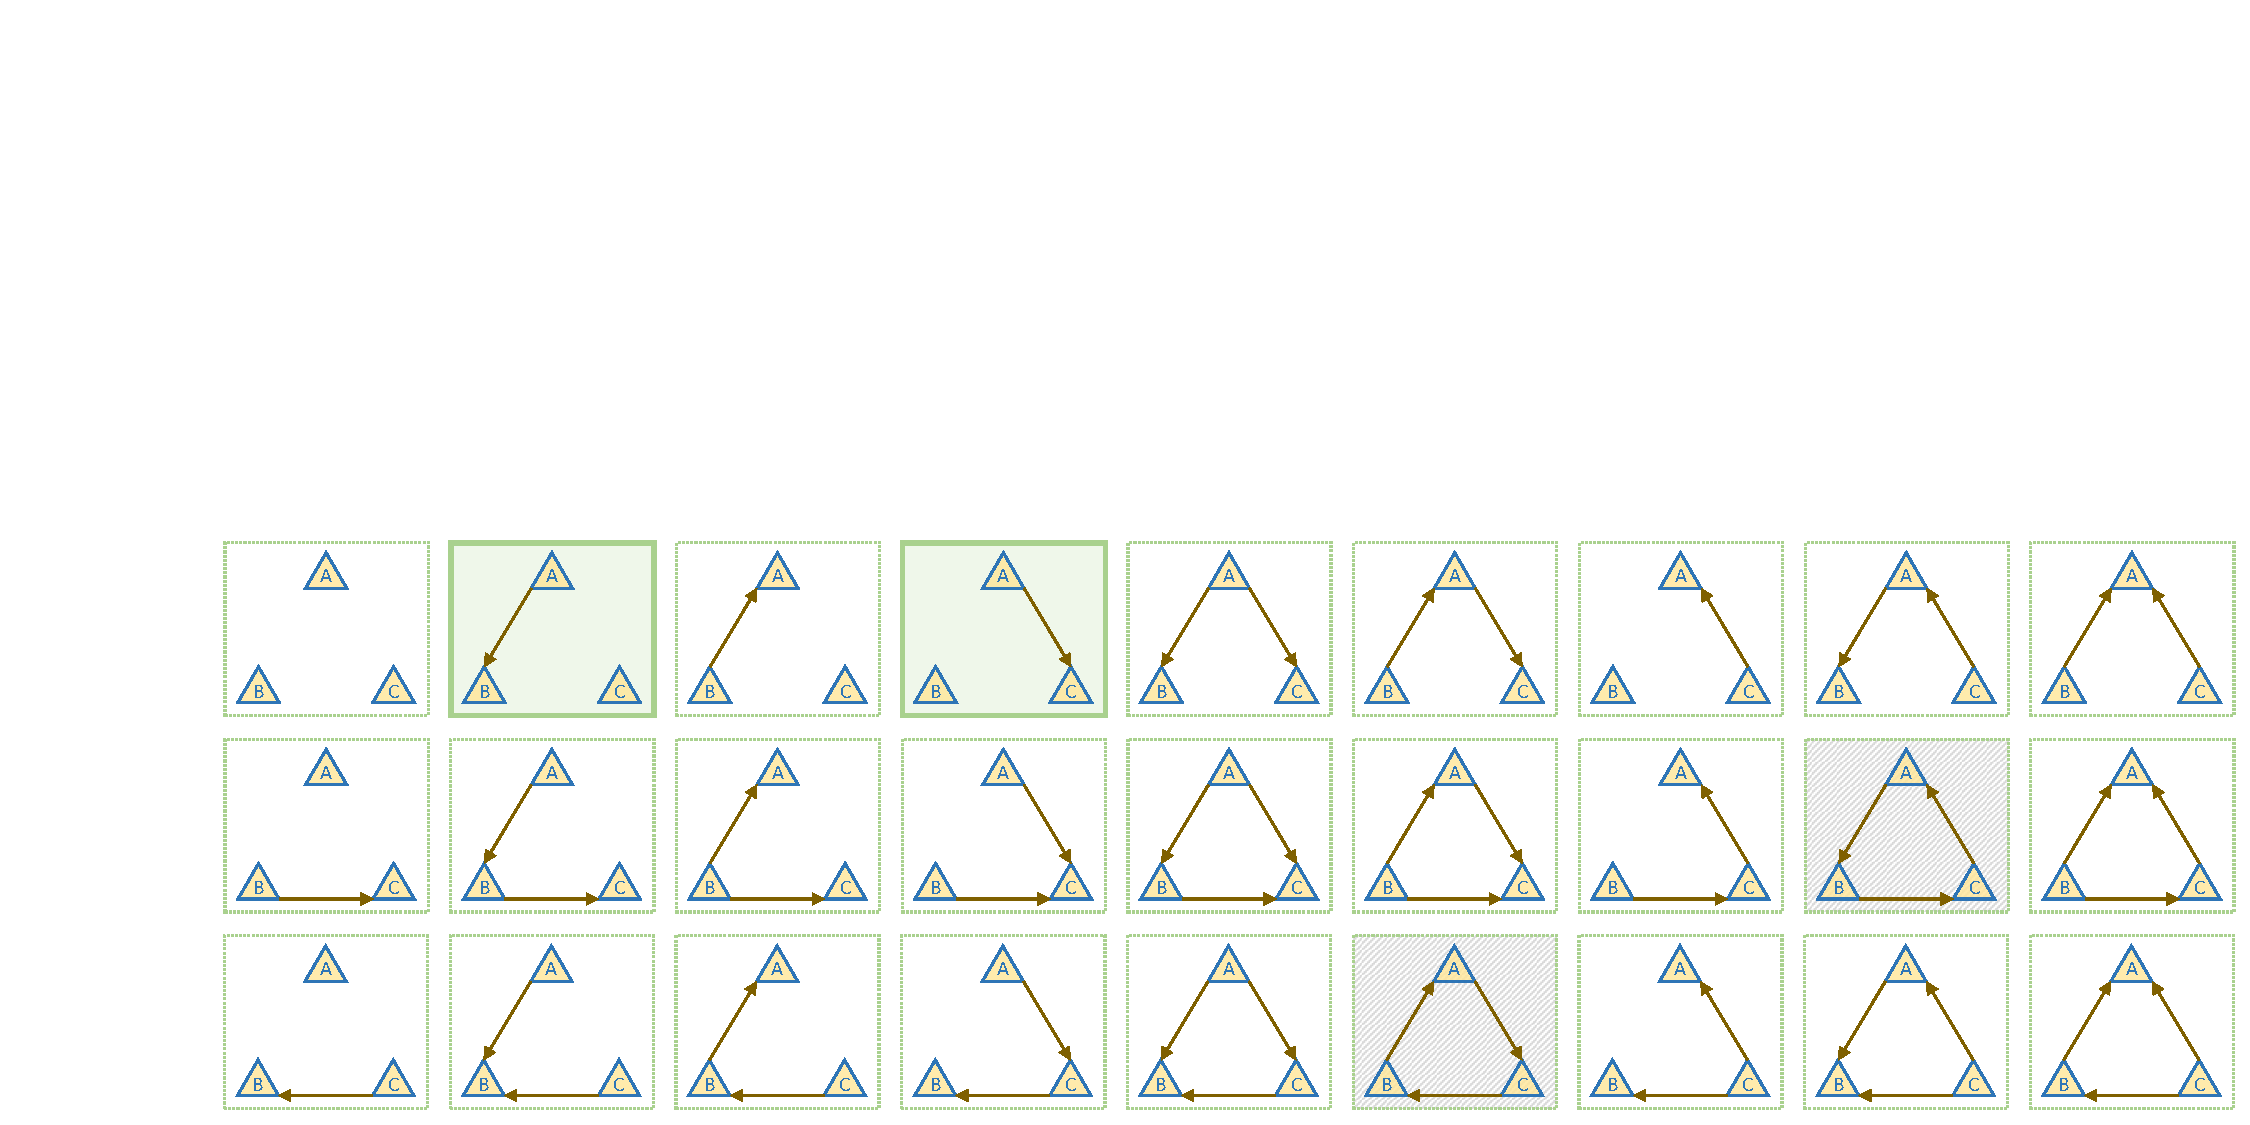
\includegraphics[clip, trim=3cm 0cm 0cm 9cm,width=\textwidth]{plot/3vci.pdf}
	\caption{All possible causal relations for 3 variables. Grey shaded blocks have causal loops (and are typically not considered). Green shaded set of blocks indicate a case of causal hypothesis testing.}
	\label{fig:3vci}
\end{figure*}

\subsection{Quantum computation and algorithmic information}

The synergy between quantum computation and algorithmic information has been studied extensively in \cite{sarkar2022applications}.
Two main directions were explored, that can be applied for causal inference.

In \cite{sarkar2021estimating} a global/objective view is presented, which involves quantum automata for algorithmic information.
A framework for causal inference based on algorithmic generative models is developed. 
This technique of quantum-accelerated experimental algorithmic information theory~(QEAIT) can be ubiquitously applied to diverse domains. 
Specifically for genome analysis, the problem of identifying bit strings capable of self-replication is presented. 
A new quantum circuit design of a quantum parallel universal linear bounded automata (QPULBA) model is developed.
This enables a superposition of classical models/programs to be executed, and their properties can be explored. 
The automaton prepares the universal distribution as a quantum superposition state which can be queried to estimate algorithmic properties of the causal model.

In \cite{sarkar2021qksa} a local/subjective view is presented, which involves universal reinforcement learning in quantum environments.
This theoretical framework can be applied for automated scientific modeling. 
A universal artificial general intelligence formalism is presented that can model quantum processes. 
The developed quantum knowledge seeking agent~(QKSA) is an evolutionary general reinforcement learning model for recursive self-improvement. 
It uses resource-bounded algorithmic complexity of quantum process tomography~(QPT) algorithms. 
The cost function determining the optimal strategy is implemented as a mutating gene within a quine. 
The utility function for an individual agent is based on a selected quantum distance measure between the predicted and perceived environment.

These techniques motivates our research in this paper.
Unlike quantum/classical data driven machine learning, these primitives of QEAIT and QKSA preserves the explanatory power of the model the learning converges to by exploring the space of programs on an automata model.
The QPULBA model (in QEAIT) and QPT algorithms (in QKSA) can be generalized to a causal oracle and causal tomography respectively.

\section{Causal hypothesis testing} \label{sec:causal-hypothesis-testing}

A canonical approach in causal inference is to formulate different hypotheses on the cause–effect relations and test them against each other.
This technique is typically used when there is some knowledge of the characteristic of the phenomenon that is being tested.
The complete search-space of directed graphs between events grows exponentially.
An exhaustive example of 3 variable causal relations is shown in Fig.~[\ref{fig:3vci}].
In causal hypothesis testing~(CHT) a subset of these graphs are considered as the set of hypothesis being tested against each others.
For the example, in Fig.~[\ref{fig:3vci}], we can consider, two hypothesis (shaded in green):
\begin{itemize} %[nolistsep,noitemsep]
	\item A causes B, C is independent
	\item A causes C, B is independent.
\end{itemize}

\subsection{Quantum advantage in classical causal hypothesis testing}

Quantum information enables a richer spectrum of causal relations that is not possible to access via classical statistics.
Most research in this direction is towards exploring causality in the quantum context~\cite{costa2016quantum,giarmatzi2019quantum,javidian2021quantum,bai2021quantum,bai2020efficient,bavaresco2021strict}.
Our focus in this work is specifically using the quantum formulation to provide a \textit{computational advantage with respect to a classical technique on classical data}.

This problem is studied extensively in \cite{chiribella2019quantum}.
The research analyzes the task of identifying the effect of a given input variable.
The constructed quantum strategy reduces the error probability by an exponential amount, doubling the decay rate of the error probability with the number of accesses to the relevant variables. 
This decay rate is the highest achievable rate allowed by quantum mechanics, even if one allows for exotic setups where the order of operations is indefinite.
The key ingredient of the quantum speedup is the ability to run multiple equivalent experiments in a quantum superposition.
This can be used for the detection of a causal link between two variables, and in the identification of the cause of a given variable, as well.

The set of allowed causal relationships depends on the physical theory, which determines which maps can be implemented by physical processes.
In classical physics, cause-effect relations are typically represented by conditional probability distributions, while, in quantum theory, they are described by quantum channels, i.e., completely positive trace-preserving maps transforming density matrices of system A into density matrices of system B.

\section{Problem formulation}\label{sec:prob-formulation}
Contrary to the general case considered in \cite{chiribella2019quantum}, our formulation is towards an implementable quantum circuit that is demonstrated on the Qiskit \texttt{statevector\_simulator}. 
This formulation is detailed here. We consider an equal number of input and output variables to implement a quantum circuit. 
Thus, we describe our input variables (causes) through the set $C = \{c_0, c_1,\dots, c_{k-1}\}$, while the output variables (effects) are the denoted by the set $E = \{e_0, e_1,\dots, e_{k-1}\}$.
\begin{equation}
|C| = |E| = k,
\end{equation}
where $k$ denotes the total number of causes/effects. We will also consider the simplification that all variables are of equal length $d = |c_i| = |e_j|$, where $c_i \in C$ and $e_j \in E$.
Thus each variable has $2^d$ states. Furthermore, we maintain the simplification that each effect is a permutation of only one cause, i.e. the map from $C$ to $E$ is a bijective function, one-to-one correspondence, or invertible function.

\subsection{Model implementation}

The practical implementation is decomposed into three following steps:
\begin{itemize}
	\item $ U_\textrm{in}^\textrm{A}, U_\textrm{in}^\textrm{B} $, represents the initialization of the system A and B respectively.
	\item $U_\textrm{per}$, decomposes into parallel strategies which represents the possible ways to partition input into pairs.
	The number of qubits in the \textit{reference} ($N_{\textrm{ref.}}$) is formulated as follows
	\begin{equation}
	N_{\textrm{ref.}} = \lceil \textrm{log}_2 (kd) \rceil,
	\end{equation}
	where $kd = N_\textrm{A}$ = $N_\textrm{B}$ represents the dimension of system A and B respectively.
	\item $U_\textrm{orc}$, represents an unknown process that induces a causal relation between input and output.
\end{itemize}
The qubit requirement of our model grows as
\begin{equation}
2N_A + \ceil{\log( N_A )}. 
\end{equation}
The model is illustrated through an implementable quantum circuit in Fig.~[\ref{fig:perm-circuit}] in Appendix.
\begin{figure*}[tbh!]
	\centering
	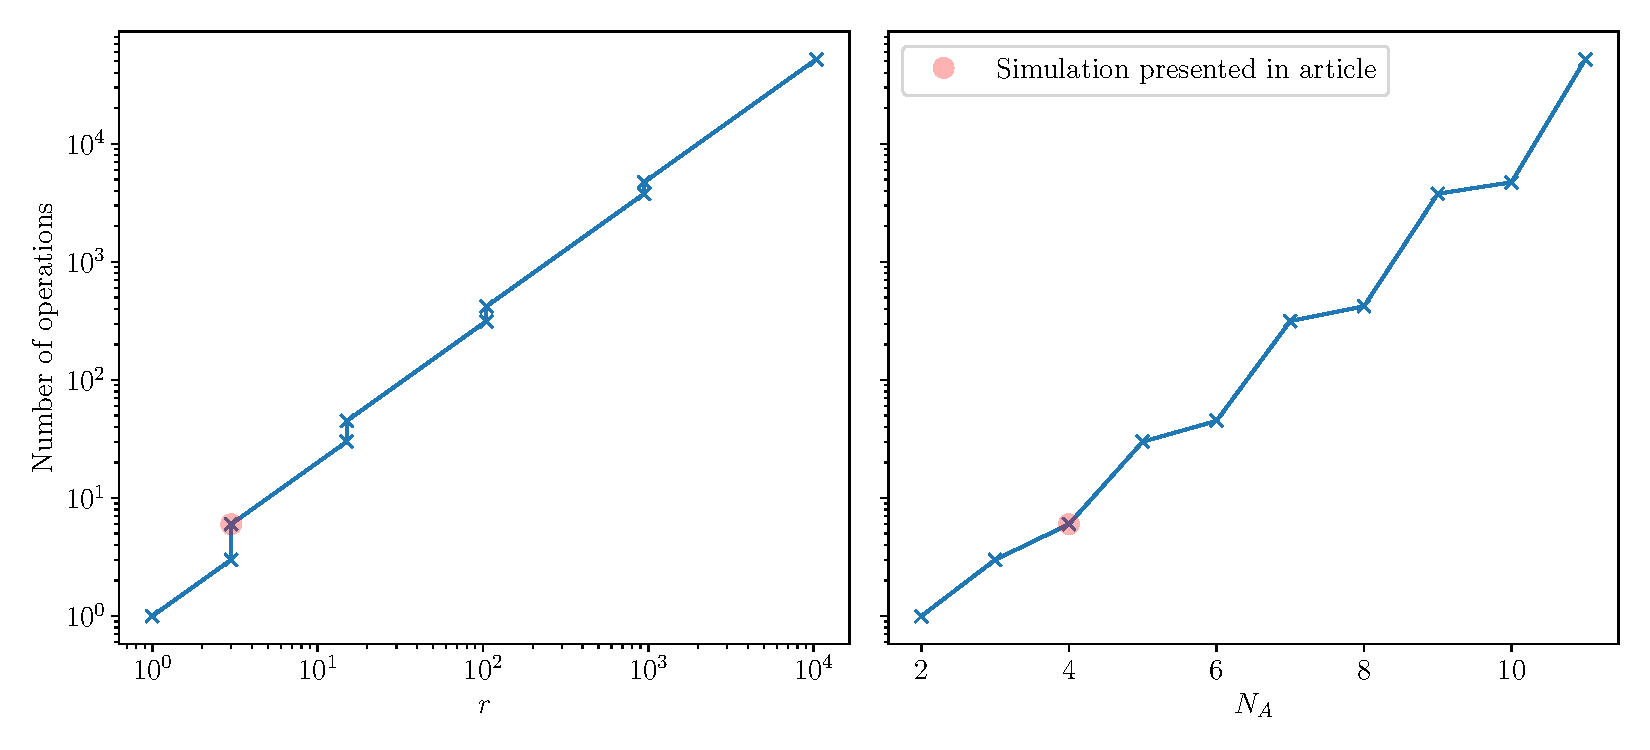
\includegraphics[width = \linewidth]{plot/number_of_operations.pdf}
	\caption{Illustration of number of controlled Bell unitary required to implement the $U_\textrm{per}$ in respect with number of linearly independent state $r$ (left hand side figure) and with the dimension of the subsystem (right hand side figure).}
	\label{fig:permutation-resource}
\end{figure*}
In the previous work one of the innovations introduced was to entangle the inputs for the parallel strategy instead of initializing with tensor product state which reduces the exponential measurement resource requirement by correlating the basis. But the cost of implementing the entangled initialization was not analysed. Through our model implementation we are able to show that the operations required to implement the $U_\textrm{per}$ grows exponentially with the dimension of the of the subsystem as illustrated in Fig.~[\ref{fig:permutation-resource}] but linear in respect with the linearly independent states i.e. $r$.
\subsection{ Practical error probability}
%----------------
\begin{figure*}
	\centering
	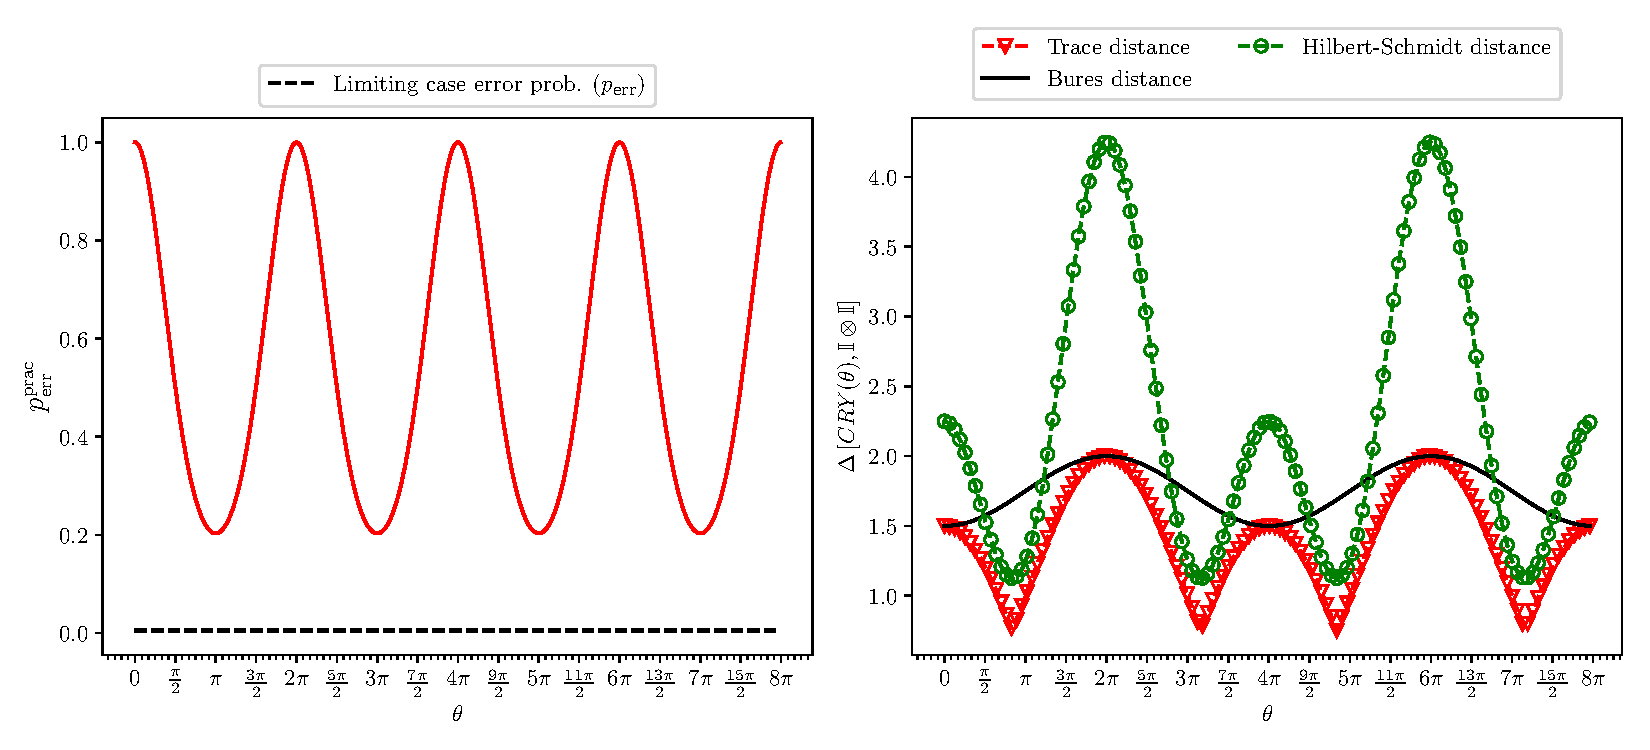
\includegraphics[width = \linewidth]{plot/limiting_error_prob.pdf}
	\caption{On the left hand side we illustrate the of variation of practical case error probability in respect with oracle parameter $\theta$. It should be noted that the default hypothesis is maximally mixed whereas the alternative hypothesis is \texttt{CRY($\theta$)}. The $x$-axis indicates the variation of the angle in \texttt{CRY($\theta$)}. On the right hand side we present the distance between the two hypothesis with $\theta$ when a class of distance measures are considered.}
	\label{fig:practical-case-error-plot}
\end{figure*}
%----------------
In quantum case the coherent superposition of equivalent configuration gives the error probability \cite{chiribella2019quantum}
\begin{equation}
p_\textrm{err} = \frac{r}{2d^N}\left( 1-\sqrt{1-r^{-2}} \right) \xrightarrow[]{r>>1}\frac{1}{4rd^N},\label{eq:limiting-case-equation}
\end{equation}
where $r$ is the number of linearly independent states. Ref.\cite{chiribella2019quantum} suggests that the Eq.\eqref{eq:limiting-case-equation} gives us the limiting case error probability. However for specific case of causal hypothesis testing the error probability should be dependent on the two specific hypothesis. As an example if $U_\textrm{orc} = U_\textrm{orc}^\textrm{alter}$ where $U_\textrm{orc}^\textrm{alter}$ is the alternate hypothesis then $p_\textrm{err} =1$.\\
From the numerical illustrations we introduce a correction factor proportional to the process distance between the two oracles. Hence the modified Eq.\eqref{eq:limiting-case-equation} takes the form
\begin{widetext}
\begin{equation}
p_\textrm{err}^\textrm{prac} = \frac{r}{2d^N}\left( 1-\sqrt{1-r^{-2}} \right)\Delta\left[U_\textrm{orc}, U_\textrm{orc}^\textrm{alter}\right] \xrightarrow[]{r>>1}\frac{\Delta\left[U_\textrm{orc}, U_\textrm{orc}^\textrm{alter}\right]}{4rd^N},\label{eq:practical-case-equation}
\end{equation}
\end{widetext}
\subsection{Numerical results}
To obtain numerical results we consider the setup represented in Fig.~[\ref{fig:perm-circuit}] where the dimension of the subsystems are same. Throughout the numerical investigation we choose the oracles as follows. $U_\textrm{orc} = \mathbb{I}^{\otimes N_\textrm{A}}\otimes \mathbb{I}^{\otimes N_\textrm{B}}$ and as for the alternate hypothesis we choose

\begin{equation}
U_\textrm{orc}^\textrm{alter}(\theta)= 
\begin{cases}
\lvert0\rangle^{\otimes N_\textrm{A}} \otimes \mathbb{I}^{\otimes N_\textrm{B}}, \\\\
\lvert1\rangle^{\otimes N_\textrm{A}} \otimes \textrm{RY}(\theta)^{\otimes N_\textrm{B}}.
\end{cases}
\label{eq:alternate-hypothesis}
\end{equation}
We have utilized IBM open-source quantum computer simulator \texttt{qiskit} and simulated the above mentioned implementation for $N_\textrm{A}=N_\textrm{B}=4$ qubits using \texttt{statevector\_simulator}. The main motivation behind the choice of \texttt{CRY$(\theta)$} as the alternate hypothesis is by varying the parameter $\theta$ one can go from non-correlated to fully correlated state.

In left hand side subfigure of Fig.~[\ref{fig:practical-case-error-plot}] we investigate the variation of error probability (see Eq.\eqref{eq:limiting-case-equation}). It can be seen that the error probability varies as
\[
p_\textrm{err} = 
\begin{cases}
p_\textrm{err}^\textrm{min}\;\;\;\;\;\;\;\;\;\;\;\;\;\;\;\;\;\;\;\;\;\;\;\;\;\;\;\;\; \textrm{for}\;\; \theta = (2m+1)\pi,\\

p_\textrm{err}^\textrm{max} \;\;\;\;\;\;\;\;\;\;\;\;\;\;\;\;\;\;\;\;\;\;\;\;\;\;\;\;\; \textrm{for}\;\; \theta = 2m\pi,\\

p_\textrm{err}^\textrm{min}<p_\textrm{err} <p_\textrm{err}^\textrm{max}\;\;\;\;\;\;\;\; \textrm{otherwise},
\end{cases}
\]
where $m=0,1,2,\ldots$. The difference in minimum error probability and the limiting case probability that is given in ref.\cite{chiribella2019quantum} is constant at
\begin{equation}
\lvert p_\textrm{err}-p_\textrm{err}^\textrm{min}\rvert\sim 0.194. 
\end{equation}
This suggests that the error probability in Eq.\eqref{eq:limiting-case-equation} requires a slight modification as per the practical implementation. This modification is reflected through the distance between the oracles under consideration i.e. $\Delta\left[U_\textrm{orc}^\textrm{alter},U_\textrm{orc}\right]$. Based on this in Eq.\eqref{eq:practical-case-equation} we introduce the practical case error probability.

Next we move forward to observe the variation of process distance in respect with oracle parameter. On the right hand side subfigure of Fig.~[\ref{fig:practical-case-error-plot}] we illustrate the distance between $U_\textrm{orc}$ and $U_\textrm{orc}^\textrm{alter}(\theta)$ in respect with $\theta$. For this investigation we have considered three distance measures
\begin{enumerate}%[noitemsep]
	\item \textit{Trace distance} which is defined by 
	\begin{equation}
	\Delta = \frac{1}{2}\textrm{Tr}\left(\rho_\textrm{orc}-\rho_\textrm{orc}^\textrm{alter}\right),
	\end{equation}
	where $\rho$ represents the Choi representation of the unitary.
	\item \textit{Bures distance} which defined as 
	\begin{equation}
	\Delta = 2\left(1-\sqrt{F(\rho_\textrm{orc},\rho_\textrm{orc}^\textrm{alter})}\right),
	\end{equation}
	where $F$ quantifies the process fidelity between the Choi representation of oracles.
	\item \textit{Hilbert-Schmidt distance} which is defined by 
	\begin{equation}
	\Delta = \textrm{Tr}\left[\left(\rho_\textrm{orc} - \rho_\textrm{orc}^\textrm{alter}\right)^2\right].
	\end{equation}
\end{enumerate}
It can be seen that the \textit{Bures} and \textit{Hilbert-Schmidt} distance coincides at $\theta=2m\pi$, where $m=0,1,2,\ldots$. 
% The numerical illustration suggests  

\section{Conclusion} \label{sec:conclusion}

In this article, we presented a quantum circuit formulation of causal tomography, as formulated in \cite{chiribella2019quantum}.
This was implemented using the open source quantum programming and simulation platform \texttt{qiskit}.
To this end, we studied stricter bounds of error probability relative to the process distance between the causal hypotheses.
We also elucidate the pragmatic gate complexity of the causal tomography entangled pair indexing. As in \cite{chiribella2019quantum} it is shown that the quantum advantage holds for generalized probabilistic theory so the practical case that we present here is optimal in any scenario.

Our motivation for this project is driven by the increasing focus on causal inference in machine learning.
Besides monitoring the information flow in future quantum communication networks, as discussed in \cite{chiribella2019quantum}, causal tomography is crucial for understanding the bounds of general intelligence and for bioinformatics use cases.
In our future work, we aim to apply our developed quantum accelerated causal tomography framework for these applications.

\begin{acknowledgments}
This project was initiated under the QIntern 2021 project ``Reinforcement Learning Agent for Quantum Foundations".
Therefore we would like to thank the organizers of the program and QWorld Association. 
We would also like to thank QIndia for providing us with a collaboration platform for the ideas motivating this research.
AK was partially supported by the Polish National Science Center (NCN) under the grant agreement $2019/33/B/ST6/02011$.
\end{acknowledgments}

\appendix

\section{Circuit Implementation}
Here we provide an illustration of the circuit that has been implemented to obtain the numerical results. Th dimension of the subsystem is kept at $4$ due to the hardware limitations.
\begin{figure*}[b!]
	\centering
	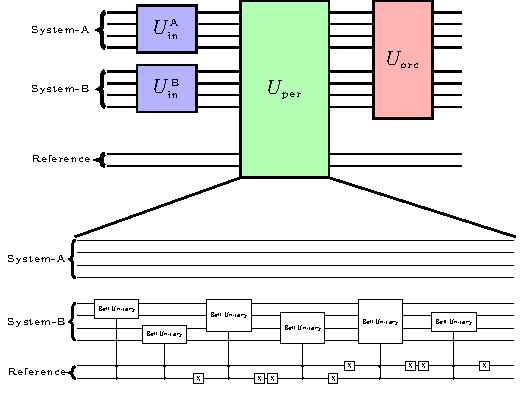
\includegraphics[width = 0.7\linewidth]{plot/bortoni.pdf}
	\caption{The illustration of the model implementation. Where we also show the decomposition of $U_\textrm{per}$ for $ N_\textrm{A} = N_\textrm{B} = 4$.}
	\label{fig:perm-circuit}
\end{figure*}

\section{Poster}
Here attach the poster which has been presented in the \texttt{Causalworlds: The interface between quantum and relativistic causality, foundations and practicalities}. The link to the conference  \href{https://causalworlds.ethz.ch/}{https://causalworlds.ethz.ch/}.
\begin{figure*}
    \centering
    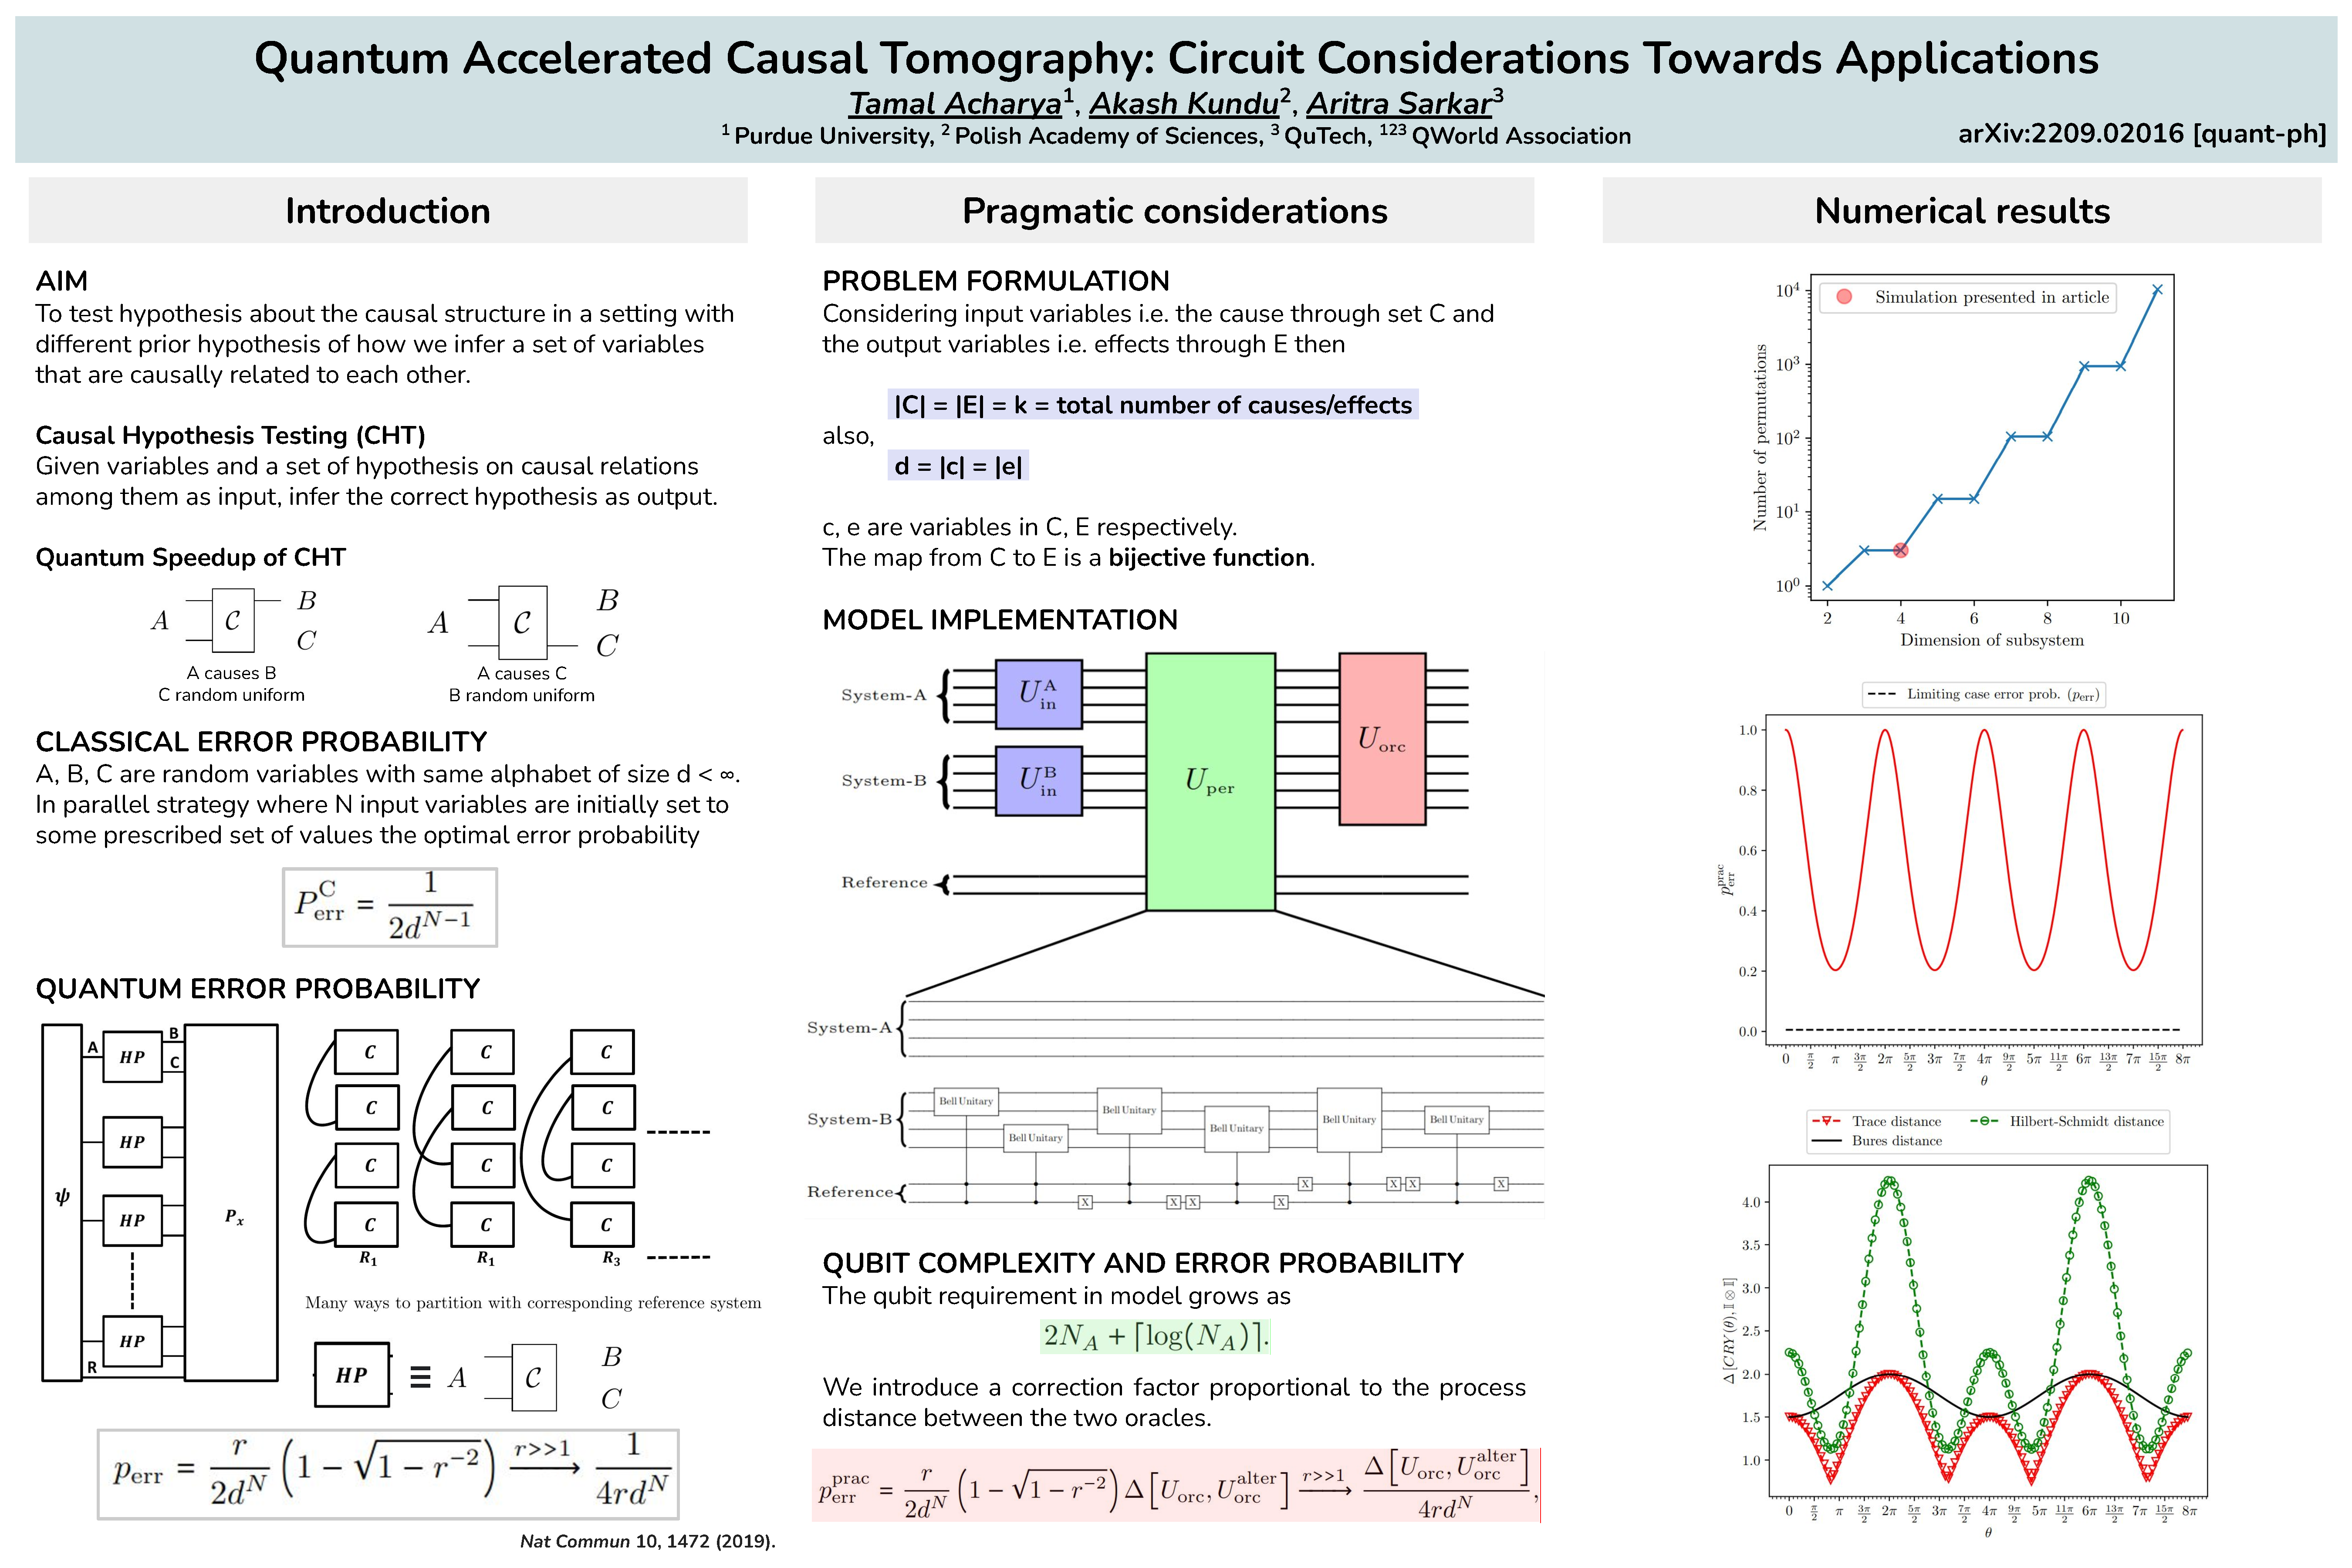
\includegraphics[width = \linewidth]{poster/practical_error_probability.pdf}
    \caption{The poster.}
    \label{fig:my_label}
\end{figure*}

\nocite{*}
\bibliography{references}% Produces the bibliography via BibTeX.

\end{document}
%
% ****** End of file aipsamp.tex ******
